\documentclass[a4paper,12pt]{article}

\usepackage[utf8]{inputenc}
\usepackage[english]{babel}
\usepackage{hyperref}
\usepackage{fontenc}
\usepackage{graphicx}
\usepackage{makeidx}
\usepackage{color}
\usepackage{multirow}
\usepackage{tabularx}
\usepackage{longtable}
\usepackage{url}
\usepackage{titlesec}
\usepackage{listings}
\usepackage{xcolor}
\usepackage{colortbl}
\usepackage{geometry}

\geometry{
    a4paper,
    left=25mm,
    right=25mm,
    top=30mm,
    bottom=30mm,
 }

%%%%%%%%%%%%%%%%%%%%%%%%%%%%%
%%%%%%% CONFIGURATION %%%%%%%
%%%%%%%%%%%%%%%%%%%%%%%%%%%%%
%%%%%%%%%%%%%%%%%%%%%%%%%%%%%%%%%%%%%%
%%%%%%% SECTION CONFIGURATIONS %%%%%%%
%%%%%%%%%%%%%%%%%%%%%%%%%%%%%%%%%%%%%%
\newcommand{\sectionbreak}{\clearpage}

\setcounter{secnumdepth}{5}

\titleformat{\paragraph}
{\normalfont\normalsize\bfseries}{\theparagraph}{1em}{}
\titlespacing*{\paragraph}
{0pt}{3.25ex plus 1ex minus .2ex}{1.5ex plus .2ex}


%%%%%%%%%%%%%%%%%%%%%%%%%%%%%%%%%%%%%%
%%%%%%% LISTINGS CONFIGURATION %%%%%%%
%%%%%%%%%%%%%%%%%%%%%%%%%%%%%%%%%%%%%%
\definecolor{mybg}{rgb}{1,1,0.8}
\definecolor{mysoftblue}{rgb}{0.6,0.729,0.867}
\definecolor{mygreen}{rgb}{0,0.6,0}
\definecolor{mygray}{rgb}{0.5,0.5,0.5}
\definecolor{mymauve}{rgb}{0.58,0,0.82}

\lstset{ %
  backgroundcolor=\color{mysoftblue},    % choose the background color; you must add \usepackage{color} or \usepackage{xcolor}
  basicstyle=\ttfamily\scriptsize,        % the size of the fonts that are used for the code
  breakatwhitespace=false,         % sets if automatic breaks should only happen at whitespace
  breaklines=true,                 % sets automatic line breaking
  captionpos=b,                    % sets the caption-position to bottom
  commentstyle=\color{mygreen},    % comment style
  deletekeywords={...},            % if you want to delete keywords from the given language
  escapeinside={\%*}{*)},          % if you want to add LaTeX within your code (example: \%* int v; *) )
  extendedchars=true,              % lets you use non-ASCII characters; for 8-bits encodings only, does not work with UTF-8
  frame=single,                    % adds a frame around the code (none, single)
  keepspaces=true,                 % keeps spaces in text, useful for keeping indentation of code (possibly needs columns=flexible)
  keywordstyle=\color{blue},       % keyword style
  language=Java,                   % the language of the code
  otherkeywords={*,...},           % if you want to add more keywords to the set
  numbers=none,                    % where to put the line-numbers; possible values are (none, left, right)
  numbersep=5pt,                   % how far the line-numbers are from the code
  numberstyle=\tiny\color{mygray}, % the style that is used for the line-numbers
  rulecolor=\color{black},         % if not set, the frame-color may be changed on line-breaks within not-black text (e.g. comments (green here))
  showspaces=false,                % show spaces everywhere adding particular underscores; it overrides 'showstringspaces'
  showstringspaces=false,          % underline spaces within strings only
  showtabs=false,                  % show tabs within strings adding particular underscores
  stepnumber=2,                    % the step between two line-numbers. If it's 1, each line will be numbered
  stringstyle=\color{mymauve},     % string literal style
  tabsize=2,                       % sets default tabsize to 2 spaces
  title=\lstname,                  % show the filename of files included with \lstinputlisting; also try caption instead of title
  aboveskip=20pt,                  % space left avobe the listing
  belowskip=0pt,                   % space left below the listing
  columns=fullflexible             % to allow automatic copy from listings
}


%%%%%%%%%%%%%%%%%%%%%%%%%%%%%%%%%%%
%%%%%%% OTHER CONFIGURATION %%%%%%%
%%%%%%%%%%%%%%%%%%%%%%%%%%%%%%%%%%%

% Horizontal line
\newcommand{\HRule}{
  \rule{\linewidth}{0.5mm}
}

% Color box for comments
\newcommand{\colorComment}[1]{
\begin{table}[h]
    \centering
    \begin{tabular}{p{0.8\textwidth}}
        \cellcolor{orange}\begin{center}
	  #1 \\
        \end{center}
        \\
    \end{tabular}
\end{table}
}
\title{COMP Superscalar}
\author{Installation Manual}
\def \compssversion {2.6}

\makeindex 

%%%%%%%%%%%%%%%%%%%%%%%%%%%%%
%%%%%%%% DOCUMENT %%%%%%%%%%%
%%%%%%%%%%%%%%%%%%%%%%%%%%%%%
\begin{document}

  %%%%%%%%%%%% TITLE PAGE %%%%%%%%%%%%%
  \hypersetup{pageanchor=false}
  \begin{titlepage} 
    \begin{center} 
      
\includegraphics[width=0.3\textwidth]{./Figures/Logos/degradado-naranja-compss.jpg}~\\[1cm] 
      \textsc{\LARGE COMP Superscalar}\\[1.5cm] 
      
      \HRule \\[0.4cm] 
      { \huge \bfseries Installation and Administration Manual \\[0.4cm] }
      \HRule \\[1.5cm] 

      { \large \textsc{Version: \compssversion}} \\[0.3cm]
      { \large \today } 
      
      \vfill 
      % Bottom of the page
      
\includegraphics[width=0.5\textwidth]{./Figures/bsc_280.jpg}~\\[1cm]
    \end{center} 
  \end{titlepage}
  \hypersetup{pageanchor=true}
  
  %%%%%%%% REFERENCE NOTES %%%%%%%%%%
  {
    This manual only provides information about how to install and configure COMPSs. Specifically, it details the installation 
    process for Debian based distributions and for RedHat based distributions, and the steps to configure COMPSs properly.
    \newline
    
    If you are not wondering to install COMPSs please consider using our already prepared \textit{Virtual Machine} available
    at our webpage: \url{http://compss.bsc.es} .
    \newline
    
    For further information about the application execution please refer to the \textit{COMPSs User Manual: Application execution
    guide} available at \url{http://compss.bsc.es/releases/compss/latest/docs/COMPSs_User_Manual_App_Exec.pdf} .
    
    For further information about the application development please refer to the \textit{COMPSs User Manual: Application development
    guide} available at \url{http://compss.bsc.es/} .
    
    For full COMPSs application examples (codes, execution commands, results, logs, etc.) please refer to the \textit{COMPSs Sample 
    Applications} available at \url{http://compss.bsc.es/releases/compss/latest/docs/COMPSs_User_Manual_App_Development.pdf} .
  }
  
  %%%%%%%% TABLE OF CONTENTS %%%%%%%%%%
  \pagenumbering{roman}
  \setcounter{tocdepth}{6}
  \tableofcontents
  \listoffigures
  \listoftables
    
  \newpage

  %%%%%%%%%%%%% CONTENTS %%%%%%%%%%%%%%
  \pagenumbering{arabic}
    
  \section{COMP Superscalar (COMPSs)}
\label{sec:Introduction}

COMP Superscalar (COMPSs) is a programming model which aims to ease the development of applications for distributed infrastructures, such as Clusters, Grids and Clouds. COMP superscalar also features a runtime system that exploits the inherent parallelism of applications at execution time.

For the sake of programming productivity, the COMPSs model has four key characteristics:

\begin{itemize}
 
 \item  {\bf Sequential programming:} COMPSs programmers do not need to deal with the typical duties of parallelization and distribution, such as thread creation and synchronization, data distribution, messaging or fault tolerance. Instead, the model is based on sequential programming, which makes it appealing to users that either lack parallel programming expertise or are looking for better programmability.
 
 \item  {\bf Infrastructure unaware:} COMPSs offers a model that abstracts the application from the underlying distributed infrastructure. Hence, COMPSs programs do not include any detail that could tie them to a particular platform, like deployment or resource management. This makes applications portable between infrastructures with diverse characteristics.
 
 \item  {\bf Standard programming languages:} COMPSs is based on the popular programming language Java, but also offers language bindings for Python and C/C++ applications. This facilitates the learning of the model, since programmers can reuse most of their previous knowledge.
 
 \item  {\bf No APIs:} In the case of COMPSs applications in Java, the model does not require to use any special API call, pragma or construct in the application; everything is pure standard Java syntax and libraries. With regard the Python and C/C++ bindings, a small set of API calls should be used on the COMPSs applications.

\end{itemize}



  \section{Packages description}
\label{sec:Packages}


\subsection{Packages structure}
Despite the fact that we recomend users to install the complete COMPSs Framework, we have built different packages to allow users
customize as maximum as possible their installation. Figure \ref{fig:compss_packages_debian} illustrates the COMPSs 
packaging structure and its internal dependencies. 
\begin{figure}[ht!]
  \centering
    \includegraphics[width=0.75\textwidth]{./Sections/2_Packages_Description/Figures/compss_packages.jpeg}
    \caption{COMPSs packaging structure}
    \label{fig:compss_packages_debian}
\end{figure}

\newpage

\subsection{Packages Dependencies}
Next we provide a list of dependencies for each COMPSs package. The exact names may vary depending on 
the Linux distribution but this list provides a general overview of the COMPSs dependencies. For specific information about
your distribution please check the \textit{Depends} section at you package manager (apt, yum, zypper, etc.).

\bgroup
  \def\arraystretch{1.5}
  \begin{center}
    \begin{tabular}{ p{6cm} | p{10cm} }
    COMPSs Framework 		& compss-runtime, compss-bindings, compss-tools, compss-cloud \\ \hline 
    COMPSs Runtime 		& compss-engine, compss-worker \\ \hline  
    COMPSs Engine 		& openjdk-7-jre, graphviz, xdg-utils \\ \hline 
    COMPSs Worker 		& openjdk-7-jre \\ \hline 
    COMPSs Bindings 		& compss-bindings-common, compss-c-binding, compss-python-binding \\ \hline 
    COMPSs Bindings Common 	& compss-engine, openjdk-7-jre \\ \hline 
    COMPSs Python Binding 	& compss-bindings-common, python ($>= 2.7$), libpython2.7 \\ \hline 
    COMPSs C/C++ Binding 	& compss-binding-common, openjdk-7-jre, automake, libtool, libboost-serialization-dev, libboost-iostreams-dev \\ \hline 
    COMPSs Tools 		& compss-extrae, compss-monitor \\ \hline 
    COMPSs Extrae 		& compss-engine, openjdk-7-jre, libxml2 ($>= 2.5$), libxml2-dev ($>= 2.5$), gfortran \\ \hline 
    COMPSs Monitor 		& compss-engine, openjdk-7-jre \\ \hline 
    COMPSs Cloud 		& compss-engine, openjdk-7-jre    
    \end{tabular}
  \end{center}
\egroup
  
  \section{Building from sources}
\label{sec:Sources}
This section describes the steps to install COMPSs from the sources.

The first step is downloading the source code from the Git repository.
\begin{lstlisting}[language=bash]
$> git clone https://github.com/bsc-wdc/compss.git
$> cd framework
\end{lstlisting}

Then, you need to download the embedded dependencies from the git submodules.
\begin{lstlisting}[language=bash]
$ framework> ./submodules_get.sh
$ framework> ./submodules_patch.sh
\end{lstlisting}

Finally you just need to run the installation script. You have to options: 
For installing COMPSs for all the users run the following command. (root access is required)
\begin{lstlisting}[language=bash]
$ framework> cd builders/
$ builders> INSTALL_DIR=/opt/COMPSs/
$ builders> sudo -E ./buildlocal [options] ${INSTALL_DIR}
\end{lstlisting}
For installing COMPSs for the current user run the following command.
\begin{lstlisting}[language=bash]
$ framework> cd builders/
$ builders> INSTALL_DIR=$HOME/opt/COMPSs/
$ builders> ./buildlocal [options] ${INSTALL_DIR}
\end{lstlisting}

The different installation options can be found in the command help.
\begin{lstlisting}[language=bash]
$ framework> cd builders/
$ builders> ./buildlocal -h
\end{lstlisting}

\subsection{Post installation}
Once your COMPSs package has been installed remember to log out and back in again to end the installation process.

If you need to set up your machine for the first time please take a look at Section \ref{sec:Additional_Configuration} for a 
detailed description of the additional configuration. 
  
  %\section{Debian-based distributions}
\label{sec:Debian}


\subsection{Prerequisites}
The commands described on the following sections require root privileges and Internet connection.

Once the installation process is finished, please log out and back in again to complete the installation. 

\subsection{Package Repository}
To add the package repository you can easily download our predefined lists by executing the following command:
\begin{lstlisting}[language=bash]
x86_64 :
   wget http://compss.bsc.es/releases/repofiles/repo_deb_x86-64.list -O /etc/apt/sources.list.d/compss-framework_x86-64.list
   
noarch :
   wget http://compss.bsc.es/releases/repofiles/repo_deb_noarch.list -O /etc/apt/sources.list.d/compss-framework_noarch.list
\end{lstlisting}

Next you need to add the repository key by executing:
\begin{lstlisting}[language=bash]
wget -qO - http://compss.bsc.es/repo/debs/deb-gpg-bsc-grid.pub.key | apt-key add -
\end{lstlisting}

And finally, refresh the apt-get repositories:
\begin{lstlisting}[language=bash]
apt-get update
\end{lstlisting}

\subsection{Installation}
Despite the fact that we recomend users to install the complete COMPSs Framework, we have built different packages to allow users
customize as maximum as possible their installation. Figure \ref{fig:compss_packages_debian} illustrates the COMPSs packaging structure.
\begin{figure}[ht!]
  \centering
    \includegraphics[width=0.75\textwidth]{./Sections/2_Debian/Figures/compss_packages.jpeg}
    \caption{COMPSs packaging structure}
    \label{fig:compss_packages_debian}
\end{figure}

\newpage
Next we describe the available packages and how to install them. 

\colorComment{If you are willing to have a full COMPSs installation just follow the COMPSs Framework instructions
and skip to next section.}

\begin{itemize}
 \item \textbf{COMPSs Framework} \newline
       Contains the all COMPSs functionalities including the Runtime, all the bindings, all the tools and the cloud connectors.
       \newline
       To install this package please run:
       \begin{lstlisting}[language=bash]
	  apt-get install compss-framework
       \end{lstlisting}
 \item \textbf{COMPSs Runtime} \newline
       Contains the COMPSs runtime to support the native functionalities. Install this package if you only need to support Java
       applications.
       \newline
       To install this package please run:
       \begin{lstlisting}[language=bash]
	  apt-get install compss-runtime
       \end{lstlisting}
       This package is composed of two sub-packages:
       \begin{itemize}
        \item \textbf{COMPSs Engine} \newline
	      Contains the COMPSs Engine, essential to run COMPSs applications as master.
	      \newline
	      To install this package please run:
	      \begin{lstlisting}[language=bash]
		  apt-get install compss-engine
	      \end{lstlisting}
        \item \textbf{COMPSs Worker} \newline
              Contains the minimum installation to allow any machine run as a COMPSs worker.
              \newline
              To install this package please run:
	      \begin{lstlisting}[language=bash]
		  apt-get install compss-worker
	      \end{lstlisting}
       \end{itemize}

 \item \textbf{COMPSs Bindings} \newline
       Contains all the bindings to support C/C++ and Python applications. 
       \newline
       To install this package please run:
       \begin{lstlisting}[language=bash]
	  apt-get install compss-bindings
       \end{lstlisting}
       This package is composed of three sub-packages:
       \begin{itemize}
        \item \textbf{COMPSs Bindings Common} \newline
	      Contains the API to allow any binding communicate with the COMPSs Runtime. It is necessary for any binding installation.
	      \newline
	      To install this package please run:
	      \begin{lstlisting}[language=bash]
		  apt-get install compss-bindings-common
	      \end{lstlisting}
        \item \textbf{COMPSs C/C++ Binding} \newline
	      Contains the C/C++ Binding
	      \newline
	      To install this package please run:
	      \begin{lstlisting}[language=bash]
		  apt-get install compss-c-binding
	      \end{lstlisting}
        \item \textbf{COMPSs Python Binding} \newline
	      Contains the Python Binding
	      \newline
	      To install this package please run:
	      \begin{lstlisting}[language=bash]
		  apt-get install compss-python-binding
	      \end{lstlisting}
       \end{itemize}

 \item \textbf{COMPSs Tools} \newline
       Contains all the COMPSs Tools.
       \newline
       To install this package please run:
       \begin{lstlisting}[language=bash]
	  apt-get install compss-tools
       \end{lstlisting}
       This package is composed of three sub-packages:
       \begin{itemize}
        \item \textbf{COMPSs Extrae} \newline
	      Contains the COMPSs Extrae tool needed to generate and process application traces.
	      \newline
	      To install this package please run:
	      \begin{lstlisting}[language=bash]
		  apt-get install compss-extrae
	      \end{lstlisting}
        \item \textbf{COMPSs Monitor} \newline
              Contains the COMPSs Monitor tool needed to monitor the application execution. 
              \newline
	      To install this package please run:
	      \begin{lstlisting}[language=bash]
		  apt-get install compss-monitor
	      \end{lstlisting}
       \end{itemize}

 \item \textbf{COMPSs Cloud} \newline
       Contains all the COMPSs Connectors needed to interact with the Cloud.
       \newline
       To install this package please run:
       \begin{lstlisting}[language=bash]
	  apt-get install compss-cloud
       \end{lstlisting}
\end{itemize} 

\subsection{Post installation}
Once your COMPSs package has been installed remember to log out and back in again to end the installation process.

If you need to setup your machine for the first time please take a look at Section \ref{sec:Additional_Configuration} for a 
detailed description of the additional configuration. 
          
  %\section{Suse-based distributions (zypper)}
\label{sec:Suse_zypper}


\subsection{Prerequisites}
The commands described on the following sections require root privileges and Internet connection.

Once the installation process is finished, please log out and back in again to complete the installation. 

\subsection{Package Repository}
To add the package repository you can easily download our predefined lists by executing the following command:
\begin{lstlisting}[language=bash]
x86_64      :  zypper addrepo -f http://compss.bsc.es/repo/rpms/stable/suse/x86_64 compss
noarch      :  zypper addrepo -f http://compss.bsc.es/repo/rpms/stable/suse/noarch compss
\end{lstlisting}

And finally, refresh the repositories:
\begin{lstlisting}[language=bash]
zypper refresh
\end{lstlisting}

\subsection{Installation}
This section describes how to install all the available COMPSs packages. If you are willing to have a full COMPSs installation 
just follow the COMPSs Framework instructions and skip directly to next section.

\begin{itemize}
 \item \textbf{COMPSs Framework} \newline
       Contains the all COMPSs functionalities including the Runtime, all the bindings, all the tools and the cloud connectors.
       \newline
       To install this package please run:
       \begin{lstlisting}[language=bash]
	  zypper install compss-framework
       \end{lstlisting}
 \item \textbf{COMPSs Runtime} \newline
       Contains the COMPSs runtime to support the native functionalities. Install this package if you only need to support Java
       applications.
       \newline
       To install this package please run:
       \begin{lstlisting}[language=bash]
	  zypper install compss-runtime
       \end{lstlisting}
       This package is composed of two sub-packages:
       \begin{itemize}
        \item \textbf{COMPSs Engine} \newline
	      Contains the COMPSs Engine, essential to run COMPSs applications as master.
	      \newline
	      To install this package please run:
	      \begin{lstlisting}[language=bash]
		  zypper install compss-engine
	      \end{lstlisting}
        \item \textbf{COMPSs Worker} \newline
             Contains the minimum installation required to run a machine as a COMPSs worker.
              \newline
              To install this package please run:
	      \begin{lstlisting}[language=bash]
		  zypper install compss-worker
	      \end{lstlisting}
       \end{itemize}

 \item \textbf{COMPSs Bindings} \newline
       Contains all the required bindings for C/C++ and Python applications.
       \newline
       To install this package please run:
       \begin{lstlisting}[language=bash]
	  zypper install compss-bindings
       \end{lstlisting}
       This package is composed of three sub-packages:
       \begin{itemize}
        \item \textbf{COMPSs Bindings Common} \newline
		  Contains the API required for the communication between any binding and the COMPSs Runtime. It is necessary for any binding installation.
	      \newline
	      To install this package please run:
	      \begin{lstlisting}[language=bash]
		  zypper install compss-bindings-common
	      \end{lstlisting}
        \item \textbf{COMPSs C/C++ Binding} \newline
	      Contains the C/C++ Binding
	      \newline
	      To install this package please run:
	      \begin{lstlisting}[language=bash]
		  zypper install compss-c-binding
	      \end{lstlisting}
        \item \textbf{COMPSs Python Binding} \newline
	      Contains the Python Binding
	      \newline
	      To install this package please run:
	      \begin{lstlisting}[language=bash]
		  zypper install compss-python-binding
	      \end{lstlisting}
       \end{itemize}

 \item \textbf{COMPSs Tools} \newline
       Contains all the COMPSs Tools.
       \newline
       To install this package please run:
       \begin{lstlisting}[language=bash]
	  zypper install compss-tools
       \end{lstlisting}
       This package is composed of three sub-packages:
       \begin{itemize}
        \item \textbf{COMPSs Extrae} \newline
	      Contains the COMPSs Extrae tool needed to generate and process application traces.
	      \newline
	      To install this package please run:
	      \begin{lstlisting}[language=bash]
		  zypper install compss-extrae
	      \end{lstlisting}
        \item \textbf{COMPSs Monitor} \newline
              Contains the COMPSs Monitor tool needed to monitor the application execution. 
              \newline
	      To install this package please run:
	      \begin{lstlisting}[language=bash]
		  zypper install compss-monitor
	      \end{lstlisting}
       \end{itemize}

 \item \textbf{COMPSs Cloud} \newline
       Contains all the COMPSs Connectors needed to interact with the Cloud.
       \newline
       To install this package please run:
       \begin{lstlisting}[language=bash]
	  zypper install compss-cloud
       \end{lstlisting}
\end{itemize} 

\subsection{Post installation}
Once your COMPSs package has been installed remember to log out and back in again to end the installation process.

If you need to set up your machine for the first time please take a look at Section \ref{sec:Additional_Configuration} for a 
detailed description of the additional configuration. 

  
  % \section{RedHat-based distributions (yum)}
\label{sec:RedHat_yum}


\subsection{Prerequisites}
The commands described on the following sections require root privileges and Internet connection.

Once the installation process is finished, please log out and back in again to complete the installation. 

\subsection{Package Repository}
To add the package repository you can easily download our predefined lists by executing the following command:
\begin{lstlisting}[language=bash]
x86_64 :  
   wget http://compss.bsc.es/releases/repofiles/repo_rpm_centos_x86-64.repo -O /etc/yum.repos.d/compss-framework_x86-64.repo
   
noarch :
   wget http://compss.bsc.es/releases/repofile/repo_rpm_centos_noarch.repo -O /etc/yum.repos.d/compss-framework_noarch.repo
\end{lstlisting}


\subsection{Installation}
Despite the fact that we recomend users to install the complete COMPSs Framework, we have built different packages to allow users
customize as maximum as possible their installation. Figure \ref{fig:compss_packages_yum} illustrates the COMPSs packaging structure.
\begin{figure}[ht!]
  \centering
    \includegraphics[width=0.75\textwidth]{./Sections/4_RedHat_yum/Figures/compss_packages.jpeg}
    \caption{COMPSs Packaging structure}
    \label{fig:compss_packages_yum}
\end{figure}

\newpage
Next we describe the available packages and how to install them. 

\colorComment{If you are willing to have a full COMPSs installation just follow the COMPSs Framework instructions
and skip to next section.}

\begin{itemize}
 \item \textbf{COMPSs Framework} \newline
       Contains the all COMPSs functionalities including the Runtime, all the bindings, all the tools and the cloud connectors.
       \newline
       To install this package please run:
       \begin{lstlisting}[language=bash]
	  yum install compss-framework
       \end{lstlisting}
 \item \textbf{COMPSs Runtime} \newline
       Contains the COMPSs runtime to support the native functionalities. Install this package if you only need to support Java
       applications.
       \newline
       To install this package please run:
       \begin{lstlisting}[language=bash]
	  yum install compss-runtime
       \end{lstlisting}
       This package is composed of two sub-packages:
       \begin{itemize}
        \item \textbf{COMPSs Engine} \newline
	      Contains the COMPSs Engine, essential to run COMPSs applications as master.
	      \newline
	      To install this package please run:
	      \begin{lstlisting}[language=bash]
		  yum install compss-engine
	      \end{lstlisting}
        \item \textbf{COMPSs Worker} \newline
              Contains the minimum installation to allow any machine run as a COMPSs worker.
              \newline
              To install this package please run:
	      \begin{lstlisting}[language=bash]
		  yum install compss-worker
	      \end{lstlisting}
       \end{itemize}

 \item \textbf{COMPSs Bindings} \newline
       Contains all the bindings to support C/C++ and Python applications. 
       \newline
       To install this package please run:
       \begin{lstlisting}[language=bash]
	  yum install compss-bindings
       \end{lstlisting}
       This package is composed of three sub-packages:
       \begin{itemize}
        \item \textbf{COMPSs Bindings Common} \newline
	      Contains the API to allow any binding communicate with the COMPSs Runtime. It is necessary for any binding installation.
	      \newline
	      To install this package please run:
	      \begin{lstlisting}[language=bash]
		  yum install compss-bindings-common
	      \end{lstlisting}
        \item \textbf{COMPSs C/C++ Binding} \newline
	      Contains the C/C++ Binding
	      \newline
	      To install this package please run:
	      \begin{lstlisting}[language=bash]
		  yum install compss-c-binding
	      \end{lstlisting}
        \item \textbf{COMPSs Python Binding} \newline
	      Contains the Python Binding
	      \newline
	      To install this package please run:
	      \begin{lstlisting}[language=bash]
		  yum install compss-python-binding
	      \end{lstlisting}
       \end{itemize}

 \item \textbf{COMPSs Tools} \newline
       Contains all the COMPSs Tools.
       \newline
       To install this package please run:
       \begin{lstlisting}[language=bash]
	  yum install compss-tools
       \end{lstlisting}
       This package is composed of three sub-packages:
       \begin{itemize}
        \item \textbf{COMPSs Extrae} \newline
	      Contains the COMPSs Extrae tool needed to generate and process application traces.
	      \newline
	      To install this package please run:
	      \begin{lstlisting}[language=bash]
		  yum install compss-extrae
	      \end{lstlisting}
        \item \textbf{COMPSs Monitor} \newline
              Contains the COMPSs Monitor tool needed to monitor the application execution. 
              \newline
	      To install this package please run:
	      \begin{lstlisting}[language=bash]
		  yum install compss-monitor
	      \end{lstlisting}
       \end{itemize}

 \item \textbf{COMPSs Cloud} \newline
       Contains all the COMPSs Connectors needed to interact with the Cloud.
       \newline
       To install this package please run:
       \begin{lstlisting}[language=bash]
	  yum install compss-cloud
       \end{lstlisting}
\end{itemize} 

\subsection{Post installation}
Once your COMPSs package has been installed remember to log out and back in again to end the installation process.

If you need to setup your machine for the first time please take a look at Section \ref{sec:Additional_Configuration} for a 
detailed description of the additional configuration. 
  
  \section{Pip}
\label{sec:Pip}

\subsection{Pre-requisites}
\label{subsec:pip_prerequisites}
In order to be able to install COMPSs and PyCOMPSs with Pip the following requirements must be met:
\begin{enumerate}
 \item Have all the dependencies (excluding the COMPSs packages) mentioned in the section \ref{subsec:packages_dependencies} satisfied and Python pip.
 As an example for some distributions:
   \subitem {\bf Fedora 25} dependencies installation command:
     \begin{lstlisting}[language=bash]
       sudo dnf install -y java-1.8.0-openjdk java-1.8.0-openjdk-devel graphviz xdg-utils libtool automake python python-libs python-pip python-devel python2-decorator boost-devel boost-serialization boost-iostreams libxml2 libxml2-devel gcc gcc-c++ gcc-gfortran tcsh @development-tools redhat-rpm-config papi
       # If the libxml softlink is not created during the installation of libxml2, the COMPSs
       # installation may fail.
       # In this case, that softlink has to be created manually with the following command:
       sudo ln -s /usr/include/libxml2/libxml/ /usr/include/libxml
     \end{lstlisting}
   \subitem {\bf Ubuntu 16.04} dependencies installation command:
     \begin{lstlisting}
       sudo apt-get install -y openjdk-8-jdk graphviz xdg-utils libtool automake build-essential python2.7 libpython2.7 libboost-serialization-dev libboost-iostreams-dev  libxml2 libxml2-dev csh gfortran python-pip libpapi-dev
     \end{lstlisting}
   \subitem {\bf OpenSuse 42.2} dependencies installation command:
     \begin{lstlisting}
       sudo zypper install --type pattern -y devel_basis
       sudo zypper install -y java-1_8_0-openjdk-headless java-1_8_0-openjdk java-1_8_0-openjdk-devel graphviz xdg-utils python python-devel libpython2_7-1_0 python-decorator libtool automake  boost-devel libboost_serialization1_54_0 libboost_iostreams1_54_0  libxml2-2 libxml2-devel tcsh gcc-fortran python-pip papi libpapi
     \end{lstlisting}
   \subitem {\bf Debian 8} dependencies installation command:
     \begin{lstlisting}
        su -
        echo "deb http://ppa.launchpad.net/webupd8team/java/ubuntu xenial main" | tee /etc/apt/sources.list.d/webupd8team-java.list
        echo "deb-src http://ppa.launchpad.net/webupd8team/java/ubuntu xenial main" | tee -a /etc/apt/sources.list.d/webupd8team-java.list
        apt-key adv --keyserver hkp://keyserver.ubuntu.com:80 --recv-keys EEA14886
        apt-get update
        apt-get install oracle-java8-installer
        apt-get install graphviz xdg-utils libtool automake build-essential python python-decorator python-pip python-dev libboost-serialization1.55.0 libboost-iostreams1.55.0 libxml2 libxml2-dev libboost-dev csh gfortran papi-tools
     \end{lstlisting}
   \subitem {\bf CentOS 7} dependencies installation command:
     \begin{lstlisting}
        sudo rpm -iUvh https://dl.fedoraproject.org/pub/epel/epel-release-latest-7.noarch.rpm
        sudo yum -y update
        sudo yum install java-1.8.0-openjdk java-1.8.0-openjdk-devel graphviz xdg-utils libtool automake python python-libs python-pip python-devel python2-decorator boost-devel boost-serialization boost-iostreams libxml2 libxml2-devel gcc gcc-c++ gcc-gfortran tcsh @development-tools redhat-rpm-config papi
        sudo pip install decorator
     \end{lstlisting}
 \item Have a proper \verb|JAVA_HOME| environment variable definition. This variable must contain a valid path to a Java JDK (as a remark, it must point to a JDK, not JRE). A possible value is the following:
 \begin{lstlisting}[language=bash]
  user@machine:~> echo $JAVA_HOME
  /usr/lib64/jvm/java-openjdk/\end{lstlisting}
\end{enumerate}


\subsection{Installation}
\label{subsec:pip_installation}
Depending on the machine, the installation command may vary. Some of the possible scenarios and their proper installation command are:
\begin{enumerate}

\item Install systemwide:
 \begin{lstlisting}[language=bash]
 sudo -E pip install pycompss -v
 \end{lstlisting}
 It is recommended to restart the user session once the installation process has finished.
Alternatively, the following command sets all the COMPSs environment.
\begin{lstlisting}[language=bash]
source /etc/profile.d/compss.sh
\end{lstlisting}
However, this command should be executed in every different terminal during the current user session.

 \item Install in user home folder (.local):
 \begin{lstlisting}[language=bash]
 pip install pycompss -v
 \end{lstlisting}
 It is recommended to restart the user session once the installation process has finished.
Alternatively, the following command sets all the COMPSs environment.
\begin{lstlisting}[language=bash]
source ~/.bashrc
\end{lstlisting}
 
 \item Within a Python virtual environment:
\begin{lstlisting}[language=bash]
 pip install pycompss -v
\end{lstlisting}
In this particular case, the installation includes the necessary variables in the activate script.
So, restart the virtual environment in order to set all the COMPSs environment.

\end{enumerate}



\subsection{Configuration}
\label{subsec:pip_configuration}
The steps mentioned in Section \ref{subsec:Passwordless_ssh} must be done in order to have a functional COMPSs and PyCOMPSs installation.


\subsection{Post installation}
As mentioned in Section \ref{subsec:pip_installation}, it is recommended to restart the user session or virtual environment once the installation process has finished.


  \section{Supercomputers}
\label{sec:Supercomputers}

The COMPSs Framework can be installed in any Supercomputer by installing its packages as in a normal distribution. The packages are
ready to be reallocated so the administrators can choose the right location for the COMPSs installation. \newline

However, if the administrators are not willing to install COMPSs through the packaging system, we also provide a \textbf{COMPSs 
zipped file} containing a pre-build script to easily install COMPSs. Next subsections provide further information about this process.

\subsection{Prerequisites}
In order to successfully run the installation script some dependencies must be present on the target machine. Administrators must 
provide the correct installation and environment of the following software:
\begin{itemize}
 \item Autotools
 \item BOOST
 \item Java 7 JRE
\end{itemize}

The following environment variables must be defined:
\begin{itemize}
 \item $JAVA\_HOME$
 \item $BOOST\_CPPFLAGS$
\end{itemize}

\subsection{Installation}
To perform the COMPSs Framework installation please execute the following commands:
\begin{lstlisting}[language=bash]
 # Check out the last COMPSs release
 $ wget http://compss.bsc.es/repo/sc/stable/COMPSs_1.3.tar.gz

 # Unpackage COMPSs
 $ tar -xvzf COMPSs_1.3.tar.gz
 
 # Install COMPSs at your preferred target location
 $ cd COMPSs
 $ ./install <targetDir>
 
 # Clean downloaded files
 $ rm -r COMPSs
 $ rm COMPSs_1.3.tar.gz
\end{lstlisting}

The installation script will create a COMPSs folder inside the given $<targetDir>$ so the final COMPSs installation will be placed 
under the $<targetDir>/COMPSs$ folder. Please note that if the folder already exists it will be \textbf{automatically erased}.

~ \newline
After completing the previous steps, administrators must ensure that the nodes have passwordless ssh access. If it is not the case,
please contact the COMPSs team at $support-compss@bsc.es$.

~ \newline
The COMPSs package also provides a \textit{compssenv} file that loads the required environment to allow users work more easily
with COMPSs. Thus, after the installation process we recomend to source the $<targetDir>/COMPSs/compssenv$ into the 
users \textit{.bashrc}.

~ \newline
Once done, remember to log out and back in again to end the installation process.

\subsection{Post installation}
To check that COMPSs Framework has been successfully installed you may run:
\begin{lstlisting}[language=bash]
 # Check the COMPSs version
 $ runcompss -v
 COMPSs version 1.3
\end{lstlisting}

For queue system executions, COMPSs provides several prebuild queue scripts than can be accessible throgh the \textit{enqueue\_compss}
command. Users can check the available options by running:
\begin{lstlisting}[language=bash]
$ enqueue_compss --help
Usage: /apps/COMPSs/1.3/Runtime/scripts/user/enqueue_compss 
         [queue_system_options] [COMPSs_options] 
         application_name application_arguments

* Options:
  General:
    --help, -h                              Print this help message
  
  Queue system configuration:
    - -exec_time=<minutes>                  Expected execution time of 
                                            the application (in minutes)
                                            Default: 10
                                            
    - -num_nodes=<int>                      Number of nodes to use
                                            Default: 2
                                            
    - -num_switches=<int>                   Maximum number of different switches.
                                            Select 0 for no restrictions.
                                            Maximum nodes per switch: 18
                                            Only available for at least 4 nodes. 
                                            Default: 0 
                                            
    - -queue_system=<name>                  Queue system to use: lsf | pbs | slurm
                                            Default: lsf
    - -queue=<name>                         Queue name to submit the job. 
                                            Depends on the queue system.
                                            For example (MN3): bsc_cs | bsc_debug
                                                | debug | interactive
                                            Default: default
                                            
    - -job_dependency=<jobID>               Postpone job execution until the job
                                            dependency has ended.
                                            Default: None
                                            
    - -tasks_per_node=<int>                 Maximum number of simultaneous
                                            tasks running on a node
                                            Default: 16
                                            
    - -master_working_dir=<path>            Working directory of the application
                                            Default: .
                                            
    - -worker_working_dir=<name>            Worker directory. Use: scratch | gpfs
                                            Default: scratch
                                            
    - -tasks_in_master=<int>                Maximum number of tasks that the master
                                            node can run as worker. Cannot exceed 
                                            tasks_per_node.
                                            Default: 0
                                            
    - -network=<name>                       Communication network for transfers:
                                            default | ethernet | infiniband | data.
                                            Default: infiniband
          
          
  Runcompss delegated parameters:

  Tools enablers:
    - -graph=<bool>, - -graph, -g           Generation of the complete graph (true/false)
                                            When no value is provided it is set to true
                                            Default: false
                                            
    - -tracing=<bool>, - -tracing, -t       Generation of traces (true/false)
                                            When no value is provided it is set to true
                                            Default: false
                                            
    - -monitoring=<int>, - -monitoring, -m  Period between monitoring samples 
                                            (milliseconds)
                                            When no value is provided it is set to 2000
                                            Default: 0
                                            
  Runtime configuration options:
    - -project=<path>                       Path to the project XML file
                                            Default: /gpfs/apps/MN3/COMPSs/1.3/Runtime/
                                            configuration/xml/projects/project.xml
                                            
    - -resources=<path>                     Path to the resources XML file
                                            Default: /gpfs/apps/MN3/COMPSs/1.3/Runtime/
                                            configuration/xml/resources/resources.xml
                                            
    - -lang=<name>                          Language of the application (java/c/python)
                                            Default: java
                                            
    - -log_level=<level>, - -debug, -d      Set the debug level: off | info | debug
                                            Default: off
  Advanced options:
    - -comm=<path>                          Class that implements the adaptor 
                                            for communications
                                            Supported adaptors: 
                                            integratedtoolkit.nio.master.NIOAdaptor | 
                                            integratedtoolkit.gat.master.GATAdaptor
                                            Default: 
                                              integratedtoolkit.nio.master.NIOAdaptor
                                              
    - -library_path=<path>                  Non-standard directories to search 
                                            for libraries (e.g. Java JVM library, 
                                            Python library, C binding library) 
                                            Default: Working Directory
                                            
    - -classpath=<path>                     Path for the application classes / modules
                                            Default: Working Directory
                                            
    - -task_count=<int>                     Only for C/Python Bindings. Maximum number
                                            of different functions/methods, invoked
                                            from the application, that have been
                                            selected as tasks
                                            Default: 50
                                            
    - -uuid=<int>                           Preset an application UUID
                                            Default: Automatic random generation
                                            
    - -PyObject_conversion=<bool>           Only for Python Binding. Enable the object
                                            conversion to string when possible
                                            (true/false).
                                            Default: false
                                            
* Application name:
    For Java applications:   Fully qualified name of the application
    For C applications:      Path to the master binary
    For Python applications: Path to the .py file containing the main program
    
* Application arguments:
    Command line arguments to pass to the application. Can be empty. 
                                            
\end{lstlisting}

If none of the pre-build sub-queue scripts adapts to your infrastructure (lsf, pbs, slurm, etc.) please contact 
the COMPSs team at $support-compss@bsc.es$ to find out a solution.

~ \newline
If you are willing to test the COMPSs Framework installation you can run any of the applications available at our application 
repository \url{https://compss.bsc.es/projects/bar}. We suggest to run the java simple application following the steps listed
inside its \textit{README} file. 

~ \newline
For further information about either the installation or the usage please check the \textit{README} file inside the COMPSs package. 


           
  \section{Additional Configuration}
\label{sec:Additional_Configuration}


\subsection{Configure SSH passwordless}
\label{subsec:Passwordless_ssh}
By default, COMPSs uses SSH libraries for communication between nodes. Consequently, after COMPSs is installed on a set of machines,
the SSH keys must be configured on those machines so that COMPSs can establish passwordless connections between them. This requires
to install the OpenSSH package (if not present already) and follow these steps \textbf{in each machine}:
\begin{enumerate}
 \item Generate an SSH key pair
       \begin{lstlisting}[language=bash]
	  $ ssh-keygen -t dsa
       \end{lstlisting}
 \item Distribute the public key to all the other machines and configure it as authorized
       \begin{lstlisting}[language=bash]
          For every other available machine (MACHINE):
	  $ scp ~/.ssh/id_dsa.pub MACHINE:./myDSA.pub
	  $ ssh MACHINE "cat ./myDSA.pub >> ~/.ssh/authorized_keys; rm ./myDSA.pub"
       \end{lstlisting}
 \item Check that passwordless SSH connections are working fine
       \begin{lstlisting}[language=bash]
          For every other available machine (MACHINE):
	  $ ssh MACHINE
       \end{lstlisting}
\end{enumerate}

For example, considering the cluster shown in Figure \ref{fig:cluster}, users will have to execute the following commands
to grant free ssh access between any pair of machines:
\begin{lstlisting}[language=bash]
 me@localhost:~$ ssh-keygen -t id_dsa
 # Granting access localhost -> m1.bsc.es
 me@localhost:~$ scp ~/.ssh/id_dsa.pub user_m1@m1.bsc.es:./me_localhost.pub
 me@localhost:~$ ssh user_m1@m1.bsc.es "cat ./me_localhost.pub >> ~/.ssh/authorized_keys; rm ./me_localhost.pub"
 # Granting access localhost -> m2.bsc.es
 me@localhost:~$ scp ~/.ssh/id_dsa.pub user_m2@m2.bsc.es:./me_localhost.pub
 me@localhost:~$ ssh user_m2@m2.bsc.es "cat ./me_localhost.pub >> ~/.ssh/authorized_keys; rm ./me_localhost.pub"
 
 me@localhost:~$ ssh user_m1@m1.bsc.es
 user_m1@m1.bsc.es:~> ssh-keygen -t id_dsa
 user_m1@m1.bsc.es:~> exit
 # Granting access m1.bsc.es -> localhost
 me@localhost:~$ scp user_m1@m1.bsc.es:~/.ssh/id_dsa.pub ~/userm1_m1.pub
 me@localhost:~$ cat ~/userm1_m1.pub >> ~/.ssh/authorized_keys
 # Granting access m1.bsc.es -> m2.bsc.es
 me@localhost:~$ scp ~/userm1_m1.pub user_m2@m2.bsc.es:~/userm1_m1.pub 
 me@localhost:~$ ssh user_m2@m2.bsc.es "cat ./userm1_m1.pub >> ~/.ssh/authorized_keys; rm ./userm1_m1.pub"
 me@localhost:~$ rm ~/userm1_m1.pub
 
 me@localhost:~$ ssh user_m2@m2.bsc.es
 user_m2@m2.bsc.es:~> ssh-keygen -t id_dsa
 user_m2@m2.bsc.es:~> exit
 # Granting access m2.bsc.es -> localhost
 me@localhost:~$ scp user_m2@m1.bsc.es:~/.ssh/id_dsa.pub ~/userm2_m2.pub
 me@localhost:~$ cat ~/userm2_m2.pub >> ~/.ssh/authorized_keys
 # Granting access m2.bsc.es -> m1.bsc.es
 me@localhost:~$ scp ~/userm2_m2.pub user_m1@m1.bsc.es:~/userm2_m2.pub 
 me@localhost:~$ ssh user_m1@m1.bsc.es "cat ./userm2_m2.pub >> ~/.ssh/authorized_keys; rm ./userm2_m2.pub"
 me@localhost:~$ rm ~/userm2_m2.pub
\end{lstlisting}

\begin{figure}[h!]
  \centering
    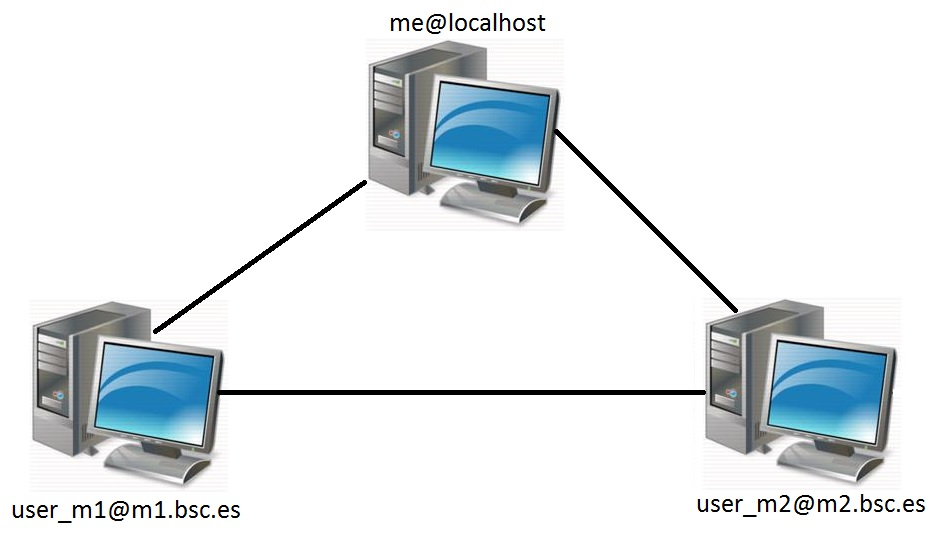
\includegraphics[width=0.95\textwidth]{./Sections/08_Additional_Configuration/Figures/cluster.jpeg}
    \caption{Cluster example}
    \label{fig:cluster}
\end{figure}


\subsection{Configure the COMPSs Cloud Connectors}
This section provides information about the additional configuration needed for some Cloud Connectors.

\subsubsection{OCCI (Open Cloud Computing Interface) connector}
In order to execute a COMPSs application using cloud resources, the rOCCI (Ruby OCCI) connector has to be configured properly.
The connector uses the rOCCI CLI client (upper versions from 4.2.5) which has to be installed in the node where the COMPSs main
application runs. The client can be installed following the instructions detailed at 
\url{http://appdb.egi.eu/store/software/rocci.cli}

  \section{Configuration Files}
\label{sec:configuration_files}

The COMPSs runtime has two configuration files: \texttt{resources.xml} and \texttt{project.xml} .
These files contain information about the execution environment and are completely independent from the application.

For each execution users can load the default configuration files or specify their custom configurations
by using, respectively, the \texttt{--resources=<absolute\_path\_to\_resources.xml>} and the
\texttt{--project=<absolute\_path\_to\_project.xml>} in the \texttt{runcompss} command. The default files are located
in the \texttt{/opt/COMPSs/Runtime/configuration/xml/} path.

Next sections describe in detail the \texttt{resources.xml} and the \texttt{project.xml} files,
explaining the available options.

\subsection{Resources file}
The \texttt{resources} file provides information about all the available resources that can be used for an execution.
This file should normally be managed by the system administrators. Its full definition schema can be found at \\
\texttt{/opt/COMPSs/Runtime/configuration/xml/resources/resource\_schema.xsd}.

For the sake of clarity, users can also check the SVG schema located at \\
\texttt{/opt/COMPSs/Runtime/configuration/xml/resources/resource\_schema.svg}.

This file contains one entry per available resource defining its name and its capabilities. Administrators can define several
resource capabilities (see example in the next listing) but we would like to underline the importance of
\textbf{ComputingUnits}. This capability represents the number of available cores in the described resource and it is
used to schedule the correct number of tasks. Thus, it becomes essential to define it accordingly to the number of cores
in the physical resource.

\begin{lstlisting}[language=xml,moredelim={[is][\textcolor{red}]{@@}{@@}}]
compss@bsc:~$ cat /opt/COMPSs/Runtime/configuration/xml/resources/default_resources.xml
<?xml version="1.0" encoding="UTF-8" standalone="yes"?>
<ResourcesList>
    <ComputeNode Name="localhost">
        <Processor Name="P1">
            @@<ComputingUnits>4</ComputingUnits>@@
            <Architecture>amd64</Architecture>
            <Speed>3.0</Speed>
        </Processor>
        <Processor Name="P2">
            @@<ComputingUnits>2</ComputingUnits>@@
        </Processor>
        <Adaptors>
            <Adaptor Name="es.bsc.compss.nio.master.NIOAdaptor">
                <SubmissionSystem>
                    <Interactive/>
                </SubmissionSystem>
                <Ports>
                    <MinPort>43001</MinPort>
                    <MaxPort>43002</MaxPort>
                </Ports>
            </Adaptor>
        </Adaptors>
        <Memory>
            <Size>16</Size>
        </Memory>
        <Storage>
            <Size>200.0</Size>
        </Storage>
        <OperatingSystem>
            <Type>Linux</Type>
            <Distribution>OpenSUSE</Distribution>
        </OperatingSystem>
        <Software>
            <Application>Java</Application>
            <Application>Python</Application>
        </Software>
    </ComputeNode>
</ResourcesList>
\end{lstlisting}


\subsection{Project file}
The project file provides information about the resources used in a specific execution. Consequently, the resources that
appear in this file are a subset of the resources described in the \texttt{resources.xml} file. This file, that contains
one entry per worker, is usually edited by the users and changes from execution to execution. Its full definition
schema can be found at
\texttt{/opt/COMPSs/Runtime/configuration/xml/projects/project\_schema.xsd}.

For the sake of clarity, users can also check the SVG schema located at \\
\texttt{/opt/COMPSs/Runtime/configuration/xml/projects/project\_schema.xsd}.

We emphasize the importance of correctly defining the following entries:
\begin{description}
 \item [installDir] Indicates the path of the COMPSs installation \textbf{inside the resource} (not necessarily the same
 than in the local machine).
 \item [User] Indicates the username used to connect via ssh to the resource. This user \textbf{must} have passwordless access to the
 resource (for more information check the \textit{COMPSs Installation Manual} available at our website \url{http://compss.bsc.es}).
 If left empty COMPSs will automatically try to access the resource with the \textbf{same username than the one that lauches
 the COMPSs main application}.
 \item [LimitOfTasks] The maximum number of tasks that can be simultaneously scheduled to a resource. Considering that a task
 can use more than one core of a node, this value must be lower or equal to the number of available cores in the resource.
\end{description}


\begin{lstlisting}[language=xml,moredelim={[is][\textcolor{red}]{@@}{@@}}]
compss@bsc:~$ cat /opt/COMPSs/Runtime/configuration/xml/projects/default_project.xml
<?xml version="1.0" encoding="UTF-8" standalone="yes"?>
<Project>
    <!-- Description for Master Node -->
    <MasterNode\>

    <!--Description for a physical node-->
    <ComputeNode Name="localhost">
        @@<InstallDir>/opt/COMPSs/</InstallDir>@@
        <WorkingDir>/tmp/Worker/</WorkingDir>
        <Application>
            <AppDir>/home/user/apps/</AppDir>
            <LibraryPath>/usr/lib/</LibraryPath>
            <Classpath>/home/user/apps/jar/example.jar</Classpath>
            <Pythonpath>/home/user/apps/</Pythonpath>
        </Application>
        @@<LimitOfTasks>4</LimitOfTasks>@@
        <Adaptors>
            <Adaptor Name="es.bsc.compss.nio.master.NIOAdaptor">
                <SubmissionSystem>
                    <Interactive/>
                </SubmissionSystem>
                <Ports>
                    <MinPort>43001</MinPort>
                    <MaxPort>43002</MaxPort>
                </Ports>
                @@<User>user</User>@@
            </Adaptor>
        </Adaptors>
    </ComputeNode>
</Project>
\end{lstlisting}
\label{lstlisting:project.xml}


\subsection{Configuration examples}
In the next subsections we provide specific information about the services, shared disks, cluster and cloud configurations and several \texttt{project.xml} and \texttt{resources.xml} examples.

\subsubsection{Parallel execution on one single process configuration}
The most basic execution that COMPSs supports is using no remote workers and running all the tasks internally within the same process that hosts the application execution. To enable the parallel execution of the application, the user needs to set up the runtime and provide a description of the resources available on the node. For that purpose, the user describes within the \texttt{<MasterNode>} tag of the \texttt{project.xml} file the resources in the same way it describes other nodes' resources on the using the \texttt{resources.xml} file. Since there is no inter-process communication, adaptors description is not allowed. In the following example, the master will manage the execution of tasks on the MainProcessor CPU of the local node - a quad-core amd64 processor at 3.0GHz - and use up to 16 GB of RAM memory and 200 GB of storage.

\begin{lstlisting}[language=xml]
<?xml version="1.0" encoding="UTF-8" standalone="yes"?>
<Project>
    <MasterNode>
        <Processor Name="MainProcessor">
            <ComputingUnits>4</ComputingUnits>
            <Architecture>amd64</Architecture>
            <Speed>3.0</Speed>
        </Processor>
        <Memory>
            <Size>16</Size>
        </Memory>
        <Storage>
            <Size>200.0</Size>
        </Storage>
    </MasterNode>
</Project>
\end{lstlisting}

If no other nodes are available, the list of resources on the \texttt{resources.xml} file is empty as shown in the following file sample. Otherwise, the user can define other nodes besides the master node as described in the following section, and the runtime system will orchestrate the task execution on both the local process and on the configured remote nodes.
~ \newline 
\begin{lstlisting}[language=xml]
<?xml version="1.0" encoding="UTF-8" standalone="yes"?>
<ResourcesList>
</ResourcesList>
\end{lstlisting}

\subsubsection{Cluster and grid configuration (static resources)}
In order to use external resources to execute the applications, the following steps have to be followed:

\begin{enumerate}
 \item Install the \textit{COMPSs Worker} package (or the full \textit{COMPSs Framework} package) on all the new
 resources following the \textit{Installation manual} available at \url{http://compss.bsc.es} .
 \item Set SSH passwordless access to the rest of the remote resources.
 \item Create the \textit{WorkingDir} directory in the resource (remember this path because it is needed
 for the \texttt{project.xml} configuration).
 \item Manually deploy the application on each node.
\end{enumerate}

The \texttt{resources.xml} and the \texttt{project.xml} files must be configured accordingly.
Here we provide examples about configuration files for Grid and Cluster environments.

~ \newline

\begin{lstlisting}[language=xml]
<?xml version="1.0" encoding="UTF-8" standalone="yes"?>
<ResourcesList>
    <ComputeNode Name="hostname1.domain.es">
        <Processor Name="MainProcessor">
            <ComputingUnits>4</ComputingUnits>
        </Processor>
        <Adaptors>
            <Adaptor Name="es.bsc.compss.nio.master.NIOAdaptor">
                <SubmissionSystem>
                    <Interactive/>
                </SubmissionSystem>
                <Ports>
                    <MinPort>43001</MinPort>
                    <MaxPort>43002</MaxPort>
                </Ports>
            </Adaptor>
            <Adaptor Name="es.bsc.compss.gat.master.GATAdaptor">
                <SubmissionSystem>
                    <Batch>
                        <Queue>sequential</Queue>
                    </Batch>
                    <Interactive/>
                </SubmissionSystem>
                <BrokerAdaptor>sshtrilead</BrokerAdaptor>
            </Adaptor>
        </Adaptors>
    </ComputeNode>

    <ComputeNode Name="hostname2.domain.es">
      ...
    </ComputeNode>
</ResourcesList>
\end{lstlisting}

\newpage

\begin{lstlisting}[language=xml]
<?xml version="1.0" encoding="UTF-8" standalone="yes"?>
<Project>
    <MasterNode/>
    <ComputeNode Name="hostname1.domain.es">
        <InstallDir>/opt/COMPSs/</InstallDir>
        <WorkingDir>/tmp/COMPSsWorker1/</WorkingDir>
        <User>user</User>
        <LimitOfTasks>2</LimitOfTasks>
    </ComputeNode>
    <ComputeNode Name="hostname2.domain.es">
      ...
    </ComputeNode>
</Project>
\end{lstlisting}


\subsubsection{Shared Disks configuration example}
Configuring shared disks might reduce the amount of data transfers improving the application performance. To configure a
shared disk the users must:
\begin{enumerate}
 \item Define the shared disk and its capabilities
 \item Add the shared disk and its mountpoint to each worker
 \item Add the shared disk and its mountpoint to the master node
\end{enumerate}

Next example illustrates steps 1 and 2. The \texttt{<SharedDisk>} tag adds a new shared disk named \texttt{sharedDisk0} and the
\texttt{<AttachedDisk>} tag adds the mountpoint of a named shared disk to a specific worker.
\begin{lstlisting}[language=xml]
<?xml version="1.0" encoding="UTF-8" standalone="yes"?>
<ResourcesList>
    <SharedDisk Name="sharedDisk0">
        <Storage>
            <Size>100.0</Size>
            <Type>Persistent</Type>
        </Storage>
    </SharedDisk>

    <ComputeNode Name="localhost">
      ...
      <SharedDisks>
        <AttachedDisk Name="sharedDisk0">
          <MountPoint>/tmp/SharedDisk/</MountPoint>
        </AttachedDisk>
      </SharedDisks>
    </ComputeNode>
</ResourcesList>
\end{lstlisting}

On the other side, to add the shared disk to the \textbf{master node}, the users must edit the \texttt{project.xml} file. Next example
shows how to attach the previous \texttt{sharedDisk0} to the master node:

\newpage

\begin{lstlisting}[language=xml]
<?xml version="1.0" encoding="UTF-8" standalone="yes"?>
<Project>
    <MasterNode>
        <SharedDisks>
            <AttachedDisk Name="sharedDisk0">
                <MountPoint>/home/sharedDisk/</MountPoint>
            </AttachedDisk>
        </SharedDisks>
    </MasterNode>

    <ComputeNode Name="localhost">
      ...
    </ComputeNode>
</Project>
\end{lstlisting}

Notice that the \texttt{resources.xml} file can have multiple \texttt{SharedDisk} definitions and that the \texttt{SharedDisks}
tag (either in the \texttt{resources.xml} or in the \texttt{project.xml} files) can have multiple \texttt{AttachedDisk} childrens
to mount several shared disks on the same worker or master.

~ \newline

\subsubsection{Cloud configuration (dynamic resources)}
In order to use cloud resources to execute the applications, the following steps have to be followed:
\begin{enumerate}
 \item Prepare cloud images with the \textit{COMPSs Worker} package or the full \textit{COMPSs Framework} package installed.
 \item The application will be deployed automatically during execution but the users need to set up the configuration files to
 specify the application files that must be deployed.
\end{enumerate}

The COMPSs runtime communicates with a cloud manager by means of connectors. Each connector implements
the interaction of the runtime with a given provider's API, supporting four basic
operations: ask for the price of a certain VM in the provider, get the time needed to create a VM,
create a new VM and terminate a VM. This design allows connectors to abstract the runtime from the particular API
of each provider and facilitates the addition of new connectors for other providers.

The \texttt{resources.xml} file must contain one or more \textbf{\texttt{<CloudProvider>}} tags
that include the information about a particular provider, associated to a given connector. The tag \textbf{must} have an
attribute \textbf{Name} to uniquely identify the provider. Next example summarizes the information to be specified by the
user inside this tag.

\newpage

\begin{lstlisting}[language=xml]
<?xml version="1.0" encoding="UTF-8" standalone="yes"?>
<ResourcesList>
    <CloudProvider Name="PROVIDER_NAME">
        <Endpoint>
            <Server>https://PROVIDER_URL</Server>
            <ConnectorJar>CONNECTOR_JAR</ConnectorJar>
            <ConnectorClass>CONNECTOR_CLASS</ConnectorClass>
        </Endpoint>
        <Images>
            <Image Name="Image1">
                <Adaptors>
                    <Adaptor Name="es.bsc.compss.nio.master.NIOAdaptor">
                        <SubmissionSystem>
                            <Interactive/>
                        </SubmissionSystem>
                        <Ports>
                            <MinPort>43001</MinPort>
                            <MaxPort>43010</MaxPort>
                        </Ports>
                    </Adaptor>
                </Adaptors>
                <OperatingSystem>
                    <Type>Linux</Type>
                </OperatingSystem>
                <Software>
                    <Application>Java</Application>
                </Software>
                <Price>
                    <TimeUnit>100</TimeUnit>
                    <PricePerUnit>36.0</PricePerUnit>
                </Price>
            </Image>
            <Image Name="Image2">
                <Adaptors>
                    <Adaptor Name="es.bsc.compss.nio.master.NIOAdaptor">
                        <SubmissionSystem>
                            <Interactive/>
                        </SubmissionSystem>
                        <Ports>
                            <MinPort>43001</MinPort>
                            <MaxPort>43010</MaxPort>
                        </Ports>
                    </Adaptor>
                </Adaptors>
            </Image>
        </Images>

        <InstanceTypes>
            <InstanceType Name="Instance1">
                <Processor Name="P1">
                    <ComputingUnits>4</ComputingUnits>
                    <Architecture>amd64</Architecture>
                    <Speed>3.0</Speed>
                </Processor>
                <Processor Name="P2">
                    <ComputingUnits>4</ComputingUnits>
                </Processor>
                <Memory>
                    <Size>1000.0</Size>
                </Memory>
                <Storage>
                    <Size>2000.0</Size>
                </Storage>
            </InstanceType>
            <InstanceType Name="Instance2">
                <Processor Name="P1">
                    <ComputingUnits>4</ComputingUnits>
                </Processor>
            </InstanceType>
         </InstanceTypes>
  </CloudProvider>
</ResourcesList>
\end{lstlisting}

The \texttt{project.xml} complements the information about a provider listed in the \texttt{resources.xml} file.
This file can contain a \textbf{\texttt{<Cloud>}} tag where to specify a list of providers, each with a
\textbf{\texttt{<CloudProvider>}} tag, whose \textbf{name} attribute must match one of the providers in the
\texttt{resources.xml} file. Thus, the \texttt{project.xml} file \textbf{must} contain a subset of the providers
specified in the \texttt{resources.xml} file. Next example summarizes the information to be specified by the user
inside this \texttt{<Cloud>} tag.

\begin{lstlisting}[language=xml]
<?xml version="1.0" encoding="UTF-8" standalone="yes"?>
<Project>
    <Cloud>
        <InitialVMs>1</InitialVMs>
        <MinimumVMs>1</MinimumVMs>
        <MaximumVMs>4</MaximumVMs>
        <CloudProvider Name="PROVIDER_NAME">
            <LimitOfVMs>4</LimitOfVMs>
            <Properties>
                <Property Context="C1">
                    <Name>P1</Name>
                    <Value>V1</Value>
                </Property>
                <Property>
                    <Name>P2</Name>
                    <Value>V2</Value>
                </Property>
            </Properties>

            <Images>
                <Image Name="Image1">
                    <InstallDir>/opt/COMPSs/</InstallDir>
                    <WorkingDir>/tmp/Worker/</WorkingDir>
                    <User>user</User>
                    <Application>
                        <Pythonpath>/home/user/apps/</Pythonpath>
                    </Application>
                    <LimitOfTasks>2</LimitOfTasks>
                    <Package>
                        <Source>/home/user/apps/</Source>
                        <Target>/tmp/Worker/</Target>
                        <IncludedSoftware>
                            <Application>Java</Application>
                            <Application>Python</Application>
                        </IncludedSoftware>
                    </Package>
                    <Package>
                        <Source>/home/user/apps/</Source>
                        <Target>/tmp/Worker/</Target>
                    </Package>
                    <Adaptors>
                        <Adaptor Name="es.bsc.compss.nio.master.NIOAdaptor">
                            <SubmissionSystem>
                                <Interactive/>
                            </SubmissionSystem>
                            <Ports>
                                <MinPort>43001</MinPort>
                                <MaxPort>43010</MaxPort>
                            </Ports>
                        </Adaptor>
                    </Adaptors>
                </Image>
                <Image Name="Image2">
                    <InstallDir>/opt/COMPSs/</InstallDir>
                    <WorkingDir>/tmp/Worker/</WorkingDir>
                </Image>
            </Images>
            <InstanceTypes>
                <InstanceType Name="Instance1"/>
                <InstanceType Name="Instance2"/>
            </InstanceTypes>
        </CloudProvider>

        <CloudProvider Name="PROVIDER_NAME2">
            ...
        </CloudProvider>
    </Cloud>
</Project>
\end{lstlisting}

For any connector the Runtime is capable to handle the next list of properties:

\begin{table}[!ht]
\def\arraystretch{1.2}
\centering
\begin{tabularx}{\linewidth}{|l|X|} \hline
	\textbf{Name} &\textbf{Description} \\ \hline
	provider-user & Username to login in the provider\\ \hline
	provider-user-credential & Credential to login in the provider\\ \hline
	time-slot & Time slot\\ \hline
	estimated-creation-time & Estimated VM creation time\\ \hline
	max-vm-creation-time & Maximum VM creation time\\ \hline
\end{tabularx}
\caption{Connector supported properties in the \texttt{project.xml} file.}
\label{tab:abstract_connector_properties}
\end{table}

Additionally, for any connector based on SSH, the Runtime automatically handles the next list of properties:

\begin{table}[!ht]
\def\arraystretch{1.2}
\centering
\begin{tabularx}{\linewidth}{|l|X|} \hline
	\textbf{Name} &\textbf{Description} \\ \hline
	vm-user & User to login in the VM\\ \hline
	vm-password & Password to login in the VM\\ \hline
	vm-keypair-name & Name of the Keypair to login in the VM\\ \hline
	vm-keypair-location & Location (in the master) of the Keypair to login in the VM \\ \hline
\end{tabularx}
\caption{Properties supported by any SSH based connector in the \texttt{project.xml} file.}
\label{tab:ssh_connector_properties}
\end{table}

Finally, the next sections provide a more accurate description of each of the currently available connector and its specific properties.

%%%%%%%%%%%%
% ROCCI
%%%%%%%%%%%%
\paragraph{Cloud connectors: rOCCI}
The connector uses the rOCCI binary client\footnote{\url{https://appdb.egi.eu/store/software/rocci.cli}}
(version newer or equal than 4.2.5) which has to be installed in the node where the COMPSs main
application is executed.

This connector needs additional files providing details about the resource templates available on
each provider. This file is located under \\ \texttt{<COMPSs\_INSTALL\_DIR>/configuration/xml/templates} path. Additionally, the user must define the virtual images flavors and instance types offered by each provider;
thus, when the runtime decides the creation of a VM, the connector selects the appropriate image and
resource template according to the requirements (in terms of CPU, memory, disk, etc) by invoking the
rOCCI client through Mixins (heritable classes that override and extend the base templates).

Table \ref{tab:rOCCI_extensions} contains the rOCCI specific properties that must be defined under the \texttt{Provider} tag in
the \texttt{project.xml} file and Table \ref{tab:rOCCI_extensions} contains the specific properties that must be defined
under the \texttt{Instance} tag.

\begin{table}[!ht]
\def\arraystretch{1.2}
\centering
\begin{tabularx}{\linewidth}{|l|X|} \hline
	\textbf{Name} &\textbf{Description} \\ \hline
	auth		& Authentication method, x509 only supported \\ \hline
	user-cred	& Path of the VOMS proxy \\ \hline
	ca-path		& Path to CA certificates directory \\ \hline
	ca-file		& Specific CA filename \\ \hline
	owner		& Optional. Used by the PMES Job-Manager \\ \hline
	jobname		& Optional. Used by the PMES Job-Manager \\ \hline
	timeout		& Maximum command time \\ \hline
	username	& Username to connect to the back-end cloud provider \\ \hline
	password	& Password to connect to the back-end cloud provider \\ \hline
	voms		& Enable VOMS authentication \\ \hline
	media-type	& Media type \\ \hline
	resource	& Resource type \\ \hline
	attributes	& Extra resource attributes for the back-end cloud provider \\ \hline
	context		& Extra context for the back-end cloud provider \\ \hline
	action		& Extra actions for the back-end cloud provider \\ \hline
	mixin		& Mixin definition \\ \hline
	link		& Link \\ \hline
	trigger-action	& Adds a trigger \\ \hline
	log-to		& Redirect command logs \\ \hline
	skip-ca-check	& Skips CA checks \\ \hline
	filter		& Filters command output \\ \hline
	dump-model	& Dumps the internal model \\ \hline
	debug		& Enables the debug mode on the connector commands \\ \hline
	verbose		& Enables the verbose mode on the connector commands \\ \hline
\end{tabularx}
\caption{rOCCI extensions in the \texttt{project.xml} file.}
\label{tab:rOCCI_extensions}
\end{table}

\newpage

\bgroup
  \def\arraystretch{1.5}
  \begin{longtable}{| p{0.25\textwidth} | p{0.7\textwidth} |}
      \hline
      \textbf{Instance} 	& Multiple entries of resource templates. \\ \hline
      Type   			& Name of the resource template. It has to be the same name than in the previous files \\ \hline
      CPU    			& Number of cores \\ \hline
      Memory 			& Size in GB of the available RAM \\ \hline
      Disk   			& Size in GB of the storage \\ \hline
      Price  			& Cost per hour of the instance \\ \hline
      \caption{Configuration of the \texttt{<provider>.xml} templates file.}
      \label{tab:rOCCI_configuration}
  \end{longtable}
\egroup


%%%%%%%%%%%%
% JCLOUDS
%%%%%%%%%%%%
\paragraph{Cloud connectors: JClouds}

The JClouds connector is based on the JClouds API version \textit{1.9.1}. Table \ref{tab:jclouds_extensions} shows the extra available
options under the \textit{Properties} tag that are used by this connector.

\begin{table}[!ht]
\def\arraystretch{1.2}
\centering
\begin{tabularx}{\linewidth}{|l|X|} \hline
	\textbf{Name} &\textbf{Description} \\ \hline
	provider & Back-end provider to use with JClouds (i.e. aws-ec2) \\ \hline
\end{tabularx}
\caption{JClouds extensions in the \texttt{project.xml} file.}
\label{tab:jclouds_extensions}
\end{table}


%%%%%%%%%%%%
% DOCKER
%%%%%%%%%%%%
\paragraph{Cloud connectors: Docker}

This connector uses a Java API client from \url{https://github.com/docker-java/docker-java}, version \textit{3.0.3}. It has not additional
options. Make sure that the image/s you want to load are pulled before running COMPSs with \texttt{docker pull IMAGE}. Otherwise,
the connectorn will throw an exception.


%%%%%%%%%%%%
% MESOS
%%%%%%%%%%%%
\paragraph{Cloud connectors: Mesos}

The connector uses the v0 Java API for Mesos which has to be installed in the node where the COMPSs main application is executed.
This connector creates a Mesos framework and it uses Docker images to deploy workers, each one with an own IP address.

By default it does not use authentication and the timeout timers are set to 3 minutes (180.000 milliseconds). The list of \textbf{optional}
properties available from connector is shown in Table \ref{tab:mesos_extensions}.

\begin{table}[!ht]
\def\arraystretch{1.2}
\centering
\begin{tabularx}{\linewidth}{|l|X|} \hline
	\textbf{Name} &\textbf{Description} \\ \hline
	mesos-framework-name & Framework name to show in Mesos.\\ \hline
  mesos-woker-name & Worker names to show in Mesos.\\ \hline
  mesos-framework-hostname & Framework hostname to show in Mesos.\\ \hline
	mesos-checkpoint  & Checkpoint for the framework.\\ \hline
	mesos-authenticate & Uses authentication? (\texttt{true}/\texttt{false}) \\ \hline
	mesos-principal & Principal for authentication.\\ \hline
	mesos-secret  & Secret for authentication.\\ \hline

	mesos-framework-register-timeout & Timeout to wait for Framework to register.\\ \hline
	mesos-framework-register-timeout-units&  Time units to wait for register.\\ \hline
	mesos-worker-wait-timeout & Timeout to wait for worker to be created.\\ \hline
	mesos-worker-wait-timeout-units  & Time units for waiting creation. \\ \hline
	mesos-worker-kill-timeout  & Number of units to wait for killing a worker. \\ \hline
	mesos-worker-kill-timeout-units  & Time units to wait for killing.\\ \hline

	mesos-docker-command  & Command to use at start for each worker.\\ \hline

	mesos-containerizer  &  Containers to use: (\texttt{MESOS}/\texttt{DOCKER}) \\ \hline
  mesos-docker-network-type &  Network type to use: (\texttt{BRIDGE}/\texttt{HOST}/\texttt{USER}) \\ \hline
  mesos-docker-network-name & Network name to use for workers.\\ \hline
  mesos-docker-mount-volume & Mount volume on workers? (\texttt{true}/\texttt{false})\\ \hline
  mesos-docker-volume-host-path & Host path for mounting volume. \\ \hline
  mesos-docker-volume-container-path  & Container path to mount volume. \\ \hline
\end{tabularx}
\caption{Mesos connector options in \texttt{project.xml} file.}
\label{tab:mesos_extensions}
\end{table}

\newpage

\noindent
* TimeUnit avialable values: \texttt{DAYS}, \texttt{HOURS}, \texttt{MICROSECONDS}, \texttt{MILLISECONDS}, \texttt{MINUTES},
\texttt{NANOSECONDS}, \texttt{SECONDS}.
\subsubsection{Services configuration}
To allow COMPSs applications to use WebServices as tasks, the \texttt{resources.xml} can include a special type of resource called
\textit{Service}. For each WebService it is necessary to specify its wsdl, its name, its namespace and
its port.
\begin{lstlisting}[language=xml]
<?xml version="1.0" encoding="UTF-8" standalone="yes"?>
<ResourcesList>
    <ComputeNode Name="localhost">
      ...
    </ComputeNode>

    <Service wsdl="http://bscgrid05.bsc.es:20390/hmmerobj/hmmerobj?wsdl">
        <Name>HmmerObjects</Name>
        <Namespace>http://hmmerobj.worker</Namespace>
        <Port>HmmerObjectsPort</Port>
    </Service>
</ResourcesList>
\end{lstlisting}

When configuring the \texttt{project.xml} file it is necessary to include the service as a worker by adding an
special entry indicating only the name and the limit of tasks as shown in the following example:
\begin{lstlisting}[language=xml]
<?xml version="1.0" encoding="UTF-8" standalone="yes"?>
<Project>
    <MasterNode/>
    <ComputeNode Name="localhost">
      ...
    </ComputeNode>

    <Service wsdl="http://bscgrid05.bsc.es:20390/hmmerobj/hmmerobj?wsdl">
        <LimitOfTasks>2</LimitOfTasks>
    </Service>
</Project>
\end{lstlisting}


  
  %\section{COMPSs Removal}
\label{sec:Removal}

\subsection{How to uninstall or remove COMPSs}
COMPSs can be easily uninstalled via the \textit{Linux Packaging Tools} by running the following commands:
\begin{lstlisting}[language=bash]
Debian: apt-get remove compss-framework
RedHat (zypper): zypper remove compss-framework
RedHat (yum): yum remove compss-framework
\end{lstlisting}

Notice that some of the COMPSs packages are meta-packages and, thus, you will need to manually uninstall all the COMPSs packages
or use the autoremove tools:
\begin{lstlisting}[language=bash]
Debian: apt-get autoremove
RedHat (zypper): zypper remove --clean-deps compss-framework
RedHat (yum): yum autoremove 
\end{lstlisting}

In \textit{Debian} based distributions uninstalling COMPSs will not erase your configuration files. If you are willing to completely
remove COMPSs please remember to use the \textit{purge} option: 
\begin{lstlisting}[language=bash]
Debian: apt-get purge compss-framework
\end{lstlisting}

\subsection{How to clean repositories}
During the installation process you may have added the COMPSs repository. If you want to clean your respository list please erase
the compss list by executing the following commands:
\begin{lstlisting}[language=bash]
Debian: 
  $ rm -f /etc/apt/sources.list.d/compss-framework_*.list
  $ apt-get update
  
RedHat (zypper):
  $ zypper removerepo compss
  $ zypper refresh 
  
RedHat (yum): 
  $ rm -f /etc/yum.repos.d/compss-framework_*.repo
\end{lstlisting}
  
  %%%%%%%%%%%%% END PAGE %%%%%%%%%%%%%%
  \newpage

  \vspace*{\fill} 
  \begin{center}
    \large { Please find more details on the COMPSs framework at }
    \huge{\url{http://compss.bsc.es}}
  \end{center}    
  \vspace*{\fill} 
           
\end{document}
